\begin{figure}[H]
    \centering
    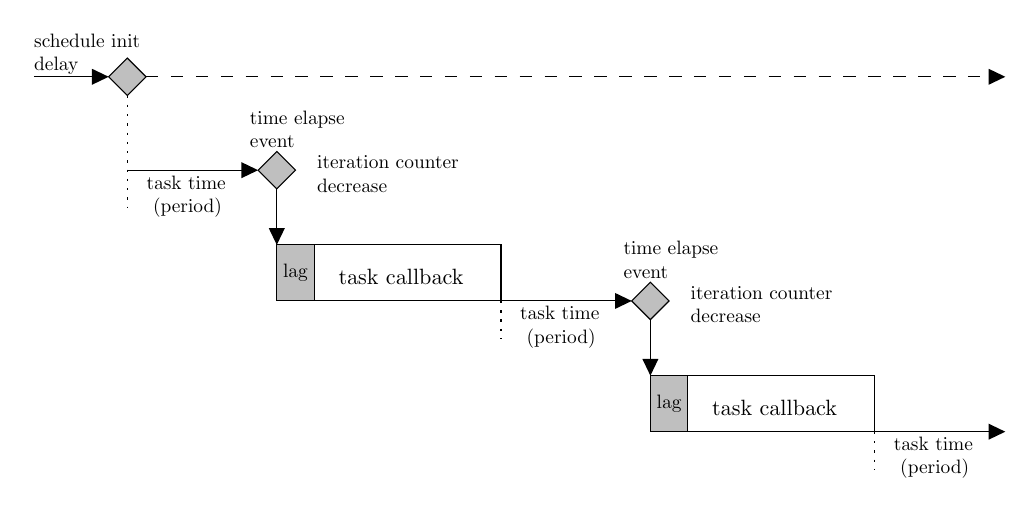
\begin{tikzpicture}[x=0.75pt,y=0.75pt,yscale=-1,xscale=1,scale=0.9]
        \draw  [fill=lightgray,fill opacity=1 ] (130,20) -- (140,30) -- (130,40) -- (120,30) -- cycle ;
        \draw    (80,30) -- (118,30) ;
        \draw [shift={(120,30)}, rotate = 180] [fill=black][line width=0.75]  [draw opacity=0] (8.93,-4.29) -- (0,0) -- (8.93,4.29) -- cycle;
        \draw  [dash pattern={on 4.5pt off 4.5pt}]  (140,30) -- (598,30) ;
        \draw [shift={(600,30)}, rotate = 180] [fill=black][line width=0.75]  [draw opacity=0] (8.93,-4.29) -- (0,0) -- (8.93,4.29) -- cycle;
        \draw  [dash pattern={on 0.84pt off 2.51pt}]  (130,40) -- (130,100) ;
        \draw    (130,80) -- (198,80) ;
        \draw [shift={(200,80)}, rotate = 180] [fill=black][line width=0.75]  [draw opacity=0] (8.93,-4.29) -- (0,0) -- (8.93,4.29) -- cycle;
        \draw  [fill=lightgray,fill opacity=1 ] (210,70) -- (220,80) -- (210,90) -- (200,80) -- cycle ;
        \draw  [fill=lightgray,fill opacity=1 ] (210,120) -- (230,120) -- (230,150) -- (210,150) -- cycle ;
        \draw   (230,120) -- (330,120) -- (330,150) -- (230,150) -- cycle ;
        \draw    (210,90) -- (210,118) ;
        \draw [shift={(210,120)}, rotate = 270] [fill=black][line width=0.75]  [draw opacity=0] (8.93,-4.29) -- (0,0) -- (8.93,4.29) -- cycle;
        \draw  [dash pattern={on 0.84pt off 2.51pt}]  (330,150) -- (330,170) ;
        \draw    (330,150) -- (398,150) ;
        \draw [shift={(400,150)}, rotate = 180] [fill=black][line width=0.75]  [draw opacity=0] (8.93,-4.29) -- (0,0) -- (8.93,4.29) -- cycle;
        \draw  [fill=lightgray,fill opacity=1 ] (410,140) -- (420,150) -- (410,160) -- (400,150) -- cycle ;
        \draw  [fill=lightgray,fill opacity=1 ] (410,190) -- (430,190) -- (430,220) -- (410,220) -- cycle ;
        \draw   (430,190) -- (530,190) -- (530,220) -- (430,220) -- cycle ;
        \draw    (410,160) -- (410,188) ;
        \draw [shift={(410,190)}, rotate = 270] [fill=black][line width=0.75]  [draw opacity=0] (8.93,-4.29) -- (0,0) -- (8.93,4.29) -- cycle;
        \draw  [dash pattern={on 0.84pt off 2.51pt}]  (530,220) -- (530,240) ;
        \draw    (530,220) -- (598,220) ;
        \draw [shift={(600,220)}, rotate = 180] [fill=black][line width=0.75]  [draw opacity=0] (8.93,-4.29) -- (0,0) -- (8.93,4.29) -- cycle;
        \draw (108.5,18) node [scale=0.7] [align=left] {schedule init\\delay};
        \draw (221,58) node [scale=0.7] [align=left] {time elapse\\event};
        \draw (220,135) node [scale=0.7] [align=left] {lag};
        \draw (276.5,137) node [scale=0.8] [align=left] {task callback};
        \draw (269.5,82) node [scale=0.7] [align=left] {iteration counter\\decrease};
        \draw (161.5,94) node [scale=0.7] [align=left] { task time\\ \ (period)};
        \draw (421,128) node [scale=0.7] [align=left] {time elapse\\event};
        \draw (420,205) node [scale=0.7] [align=left] {lag};
        \draw (476.5,207) node [scale=0.8] [align=left] {task callback};
        \draw (469.5,152) node [scale=0.7] [align=left] {iteration counter\\decrease};
        \draw (361.5,164) node [scale=0.7] [align=left] { task time\\ \ (period)};
        \draw (561.5,234) node [scale=0.7] [align=left] { task time\\ \ (period)};
    \end{tikzpicture}
    \caption{Inherit time lag}
    \label{fig:timelag}
\end{figure}